\documentclass[a4paper,french]{paper}
\usepackage{../../_latex_assets/villemejane_iogs_ceti}

%Informations about this document 
%------------------------------------------
\def\module{Ingénierie Electronique pour le Traitement de l'Information}
\def\moduleAbrege{6N-047-SCI / IéTI}
\def\annee{}

\def\titre{TD 4 / Asservir un système}
\author{Julien VILLEMEJANE}

\subtitle{TD 4}
\institution{LEnsE / Institut d'Optique Graduate School}

\title{\titre}
\begin{document} 
%Beginning First Page. 
%------------------------------------------
\enteteThematiqueObligatoire{}

%Beginning Content. 
%------------------------------------------
\vspace{-1cm}
%%%%%%%%%%%%%%%%%%%

On s'intéresse au système bouclé suivant :

\begin{center}
	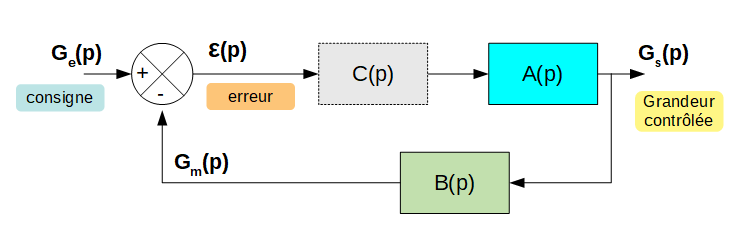
\includegraphics[width=13cm]{images/syst_asservi.png}
\end{center}

où :

\begin{itemize}
	\item $A(p)$ : système à asservir
	\item $B(p)$ : système de mesure (retour) de la grandeur à asservir
	\item $C(p)$ : correcteur de l'asservissement
	\item $G_e(p)$ : grandeur physique de consigne
	\item $G_s(p)$ : grandeur physique de sortie
	\item $\varepsilon(p)$ : erreur entre la consigne et la sortie
\end{itemize}


%%%%%%%%%%%%%%%%%%%
\encadreTDExo{1a - Boucle ouverte}{
%%%%%%%%%%%%%%%%%%%%%%%%%%%%%%%%%%%%%
Calculez la fonction de transfert en boucle ouverte : $TF_{BO}(p) = \frac{G_m(p)}{\varepsilon{}(p)}$
}	
	
%%%%%%%%%%%%%%%%%%%
\encadreTDExo{1b - Boucle fermée}{
En boucle fermée, on désire que le système :

\begin{itemize}
	\item suive la consigne en régime établi (précision)
	\item élimine les perturbations (rejet des perturbations)
	\item ait une dynamique rapide
\end{itemize}

\begin{enumerate}
	\item Calculez la fonction de transfert en boucle fermée, entre la consigne et la grandeur contrôlée : $TF_{BF}(p) = \frac{G_s(p)}{G_e(p)}$
	
	\medskip 
	
	On notera $L(p) = A(p) \cdot B(p) \cdot C(p)$.
	
	\item Que devient l'expression précédente $TF_{BF}(p)$ ?
	\item Ce système peut-il être instable ?
\end{enumerate}
}

\newpage
%%%%%%%%%%%%%%%%%%%%%%%%%%%%%%%%%%%%%
\subsection*{Stabilité d'un système}

Certains systèmes bouclés peuvent devenir instable si la fonction de transfert en boucle ouverte devient réelle (pour certaines fréquences) et de valeur inférieure à -1. En ajoutant des éléments correcteurs, il est possible de modifier le comportement et ainsi éviter que le système ne devienne instable, tout en essayant de le rendre plus rapide et plus robuste. 

Pour estimer les risques d'instabilité, on s'intéresse aux marges de gain et de phase d'un système en boucle ouverte, qui déterminera ensuite sa robustesse en boucle fermée.

Le point critique à ne pas franchir est le point -1, c'est à dire la pulsation pour laquelle $\lvert L(p) \rvert = 1 = 0dB$ et $arg(L(p)) = -\pi$. 

\qquad

\textit{Cette condition n'est pas suffisante pour garantir la stabilité d'un système bouclé. Il existe un ensemble d'autres règles permettant d'identifier cette stabilité, qui ne seront pas décrits cette année.}



%%%%%%%%%%%%%%%%%%%
\encadreTDExo{2a - Stabilité d'un système}{
%%%%%%%%%%%%%%%%%%%%%%%%%%%%%%%%%%%%%
On propose d'étudier le système dont on donne le diagramme de Bode suivant :

\begin{center}
	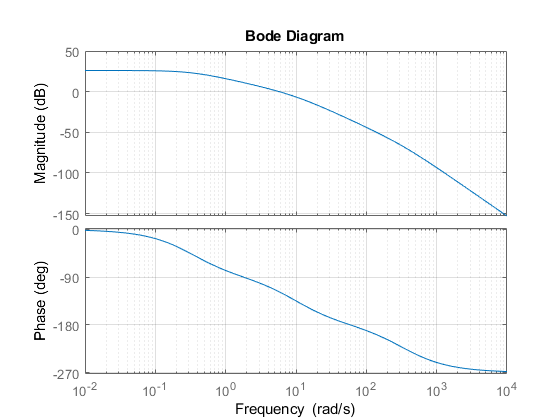
\includegraphics[width=15cm]{images/TD/sys_stable2.png}
\end{center}

Mesurez les marges de gain et de phase et concluez sur sa stabilité en boucle fermée.
}

\encadreTDExo{2b - Stabilité d'un système}{
Qu'en est-il de ce nouveau système dont on donne le diagramme de Bode ?

\begin{center}
	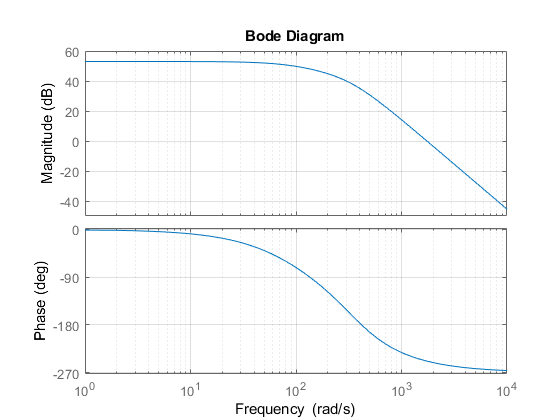
\includegraphics[width=15cm]{images/TD/sys_instable2.png}
\end{center}

}


%%%%%%%%%%%%%%%%%%%
\encadreTDExo{3a - Correction d'un système}{

Dans cette partie, on utilisera comme exemple un système du premier ordre de la forme : 

$$H(p) = \frac{H_0}{1 + \tau \cdot p}$$

On prendra $H_0 = 0.5$ et $\tau = 2 \cdot 10^{-3}$

Parmi les réponses en fréquence proposées par la suite, laquelle correspond :
\begin{enumerate}
	\item au système en boucle ouverte 
	\item au système en boucle fermée, avec un retour unitaire ($B(p) = 1$) et sans correction ($C(p) = 1$)
	\item au système en boucle fermée, avec un retour unitaire ($B(p) = 1$) et une correction proportionnelle ($C(p) = G$ avec $G = 10$)
	\item au système en boucle fermée, avec un retour unitaire ($B(p) = 1$) et une correction proportionnelle et intégrale ($C(p) = G + 1/(\tau_i \cdot p)$ avec $G = 10$ et $\tau_i = 3 \cdot 10^{-5}$)
\end{enumerate}

\begin{center}
	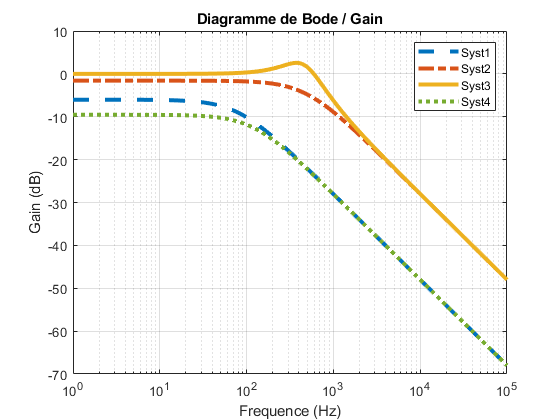
\includegraphics[width=15cm]{images/TD/sys_boucle_bode.png}
\end{center}
}

%%%%%%%%%%%%%%%%%%%
\encadreTDExo{3b - Correction d'un système}{
Même question avec les réponses indicielles suivantes.

\begin{center}
	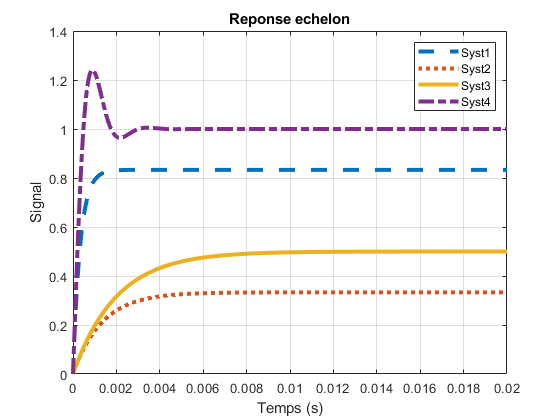
\includegraphics[width=15cm]{images/TD/sys_boucle_step.png}
\end{center}
}

%%%%%%%%%%%%%%%%%%%
\encadreTDExo{4 - Exemple de correction proportionnelle et intégrale}{

On se base sur le système précédent, $H(p) = \frac{H_0}{1 + \tau \cdot p}$, rebouclé de manière unitaire ($B(p) = 1$) et une correction proportionnelle et intégrale ($C(p) = G + 1/(\tau_i \cdot p)$ avec $G = 10$).

Précisez si la correction intégrale est bien choisie dans les 4 cas suivants (réponse indicielle et réponse fréquentielle).

\begin{center}
	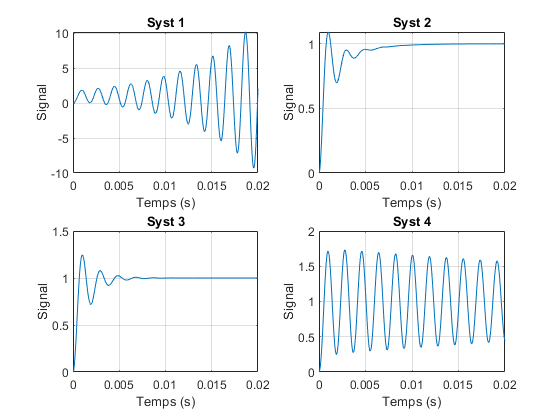
\includegraphics[width=10cm]{images/TD/sys_boucle_corrige_step.png} 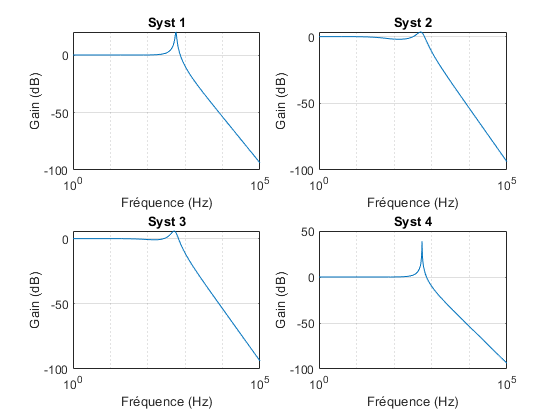
\includegraphics[width=10cm]{images/TD/sys_boucle_corrige_bode.png} 
\end{center}
}


%%%%%%%%%%%%%%%%%%%
\encadreTDExo{5 - Exemple : Amplificateur non-inverseur}{

On rappelle qu'un ALI (Amplificateur Linéaire Intégré) peut être modélisé par une fonction de transfert du premier ordre du type : 

$$A(p) = \frac{A_0}{1 + \frac{p}{\omega_0}}$$

où $A_0$ est l'amplification différentielle statique et $\omega_0 = \frac{GBP}{A_0}$ la pulsation de coupure, avec $GBP$ la bande-passante unitaire.

On réalise autour de cet ALI un montage non-inverseur, dont le schéma est donné par la suite.

\begin{center}
	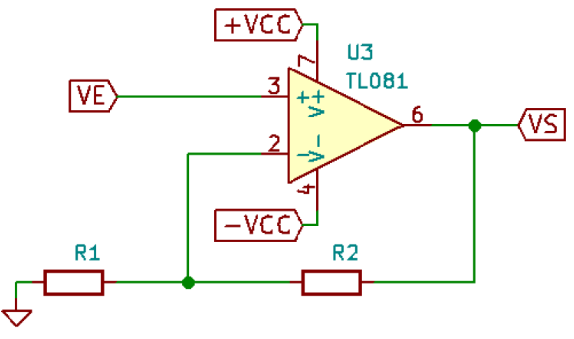
\includegraphics[width=10cm]{images/TD/noninverseur.png}
\end{center}


\begin{enumerate}
	\item Proposez un schéma bloc pour un \textbf{montage amplificateur non-inverseur}.
	\item Calculez la fonction de transfert en boucle fermée de ce montage. 
	\item Que valent à présent le gain statique et la pulsation caractéristique de ce système (pour les mêmes valeurs de $A_0$ et $GBP$) ?	
\end{enumerate}
}




\end {document}